%\thispagestyle{myheadings}
\section{Keynote Address: Ido Dagan}
\index{Dagan, Ido}

\begin{center}
\begin{Large}
{\bfseries\Large Where next? Towards multi-text consumption via three inspired research lines}\vspace{1em}\par
\end{Large}

%% \begin{center}
%%   \begin{tabular}{m{1in}b{1in}}
%%     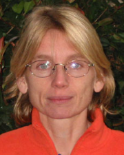
\includegraphics[width=1in]{content/monday/cortes-headshot.png}
%%     & {\bfseries Corinna Cortes} \newline Google Research, NY
%%   \end{tabular}
%% \end{center}

\daydateyear, 8:00--9:00am \vspace{1em}\\
\PlenaryLoc \\
\vspace{1em}\par
%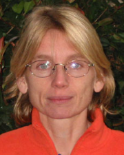
\includegraphics[height=100px]{content/monday/cortes-headshot.png}
\end{center}

\noindent
{\bfseries Abstract:} What effect does language have on people?

While the Dominican Republic is obviously my next exciting travel destination, in this talk I’ll share what I consider as exciting destinations for next steps in NLP research. I’ll start by pointing at a motivating grand application challenge: supporting effective human consumption of multi-text information -- an invaluable goal which has seen very little progress since search engine inception. I’ll then describe three individual, yet synergetic, research lines that were inspired by seeking this goal. First, supporting multi-text consumption is inherently an interactive process, where the user assists and directs the system in presenting most valuable information. As a first step, we  propose a formulation of interactive summarization, turning it into a viable and measurable research task by extending summarization evaluation methods to the interactive setting. Second, presenting scattered information in a concise and consolidated manner requires extensive methods for linking cross-text information. Promoting such a  research line, we propose several infrastructure contributions to cross-document coreference resolution, extend the scope of matching cross-text information to the interpretable levels of proposition spans and predicate-argument relations, and design a Cross-document Language Model (CDLM) which is geared for the multi-text
 setting. Lastly, we suggest that linking and consolidating multi-text information in a refined and controllable manner can benefit from some explicit interpretable representations of textual information. Rather than following traditional formal semantic representations, we propose a midway between those and opaque distributed neural representations. Text information is decomposed into a set of minimal natural language question-answer pairs, providing a generally appealing semi-structured representation for propositions in a single text, as well as a basis for aligning cross-text information units. Altogether, we advocate the promise of each individual research line for NLP progress, while suggesting human consumption of multi-text information as an inspiring research framework with a huge applied value.

\vspace{3em}\par

\vfill
\noindent

{\bfseries Biography:} Ido Dagan is a Professor at the Department of Computer Science at Bar-Ilan University, Israel, the founder of the Natural Language Processing (NLP) Lab at Bar-Ilan, the founder and head of the nationally funded Bar-Ilan University Data Science Institute, and a Fellow of the Association for Computational Linguistics (ACL). His interests are in applied semantic processing, focusing on textual inference, natural open semantic representations, consolidation and summarization of multi-text information, and interactive text summarization and exploration. Dagan and colleagues
 initiated and promoted textual entailment recognition (RTE, later aka NLI) as a generic empirical task. He was the President of the ACL in 2010 and served on its Executive Committee during 2008-2011. In that capacity, he led the establishment of the journal Transactions of the Association for Computational Linguistics, which became one of two premiere journals in NLP. Dagan received his B.A. summa cum laude and his Ph.D. (1992) in Computer Science from the Technion. He was a research fellow at the IBM Haifa Scientific Center (1991) and a Member of Technical Staff at AT&T Bell Laboratories (1992-1994). During 1998-2003 he was co-founder and CTO of FocusEngine and VP of Technology of LingoMotors, and has been regularly consulting in the industry. His academic research has involved extensive industrial collaboration, including funds from IBM, Google, Thomson-Reuters, Bloomberg, Intel and Facebook, as well as collaboration with local companies under funded projects of the Israel Innovation Authority.

\newpage
